\chapter{Introduction}

Notre projet a pour but la création d'une plateforme de gestion des mobilités de l'INSA de Rennes. Celle-ci facilitera l'affectation et le suivit des élèves en mobilité sortante. Elle permettra aussi une meilleure traçabilité des élèves, et l'obtension de données statistiques.

Vous pourrez retrouver le choix des technologies et les spécifications fonctionnelles de notre projet dans les précédents rapports. Pour rappel, notre application Web est développée en \php, à l'aide du framework \symfony. Elle utilise le système de base de données \mdb et est hébergée au Centre de Ressources Informatiques (CRI) sur un serveur \textit{Nginx}. Nous utilisons enfin le système CAS (Central Authentication Service) du CRI pour nous permettre d'authentifier les utilisateurs.

\bigbreak

Notons que notre application est déjà en cours d'utilisation. En effet, nous avions pour objectif de développer notre projet en parrallèle à la gestion des mobilités de cette année. Nous avions donc des contraintes de temps plus fortes, mais aussi de quoi tester notre application en situation réelle. Elle a ainsi été utilisée pour affecter les élèves de 3A et 4A du département informatique cette année. Nous en sommes désormais à l'implémentation de la gestion des documents nécessaires aux mobilités (notamment contrats d'étude).

\bigbreak

L'architecture de notre projet sera séparé en deux parties. Nous verrons d'abord la partie base de données, puis l'organisation des vues du site. Nous verrons ensuite comment s'articulent les différents modules utilisés.

\bigbreak
La figure \ref{useCase} est un rappel du fonctionnement habituel de l'application, et l'avancement du projet par la même occasion. Notons que les fonctionnalités en rouge ne sont pas encore implémentées, et que celles en vert sont en cours d'implémentation ou de test. 

\begin{figure}
	\centering
	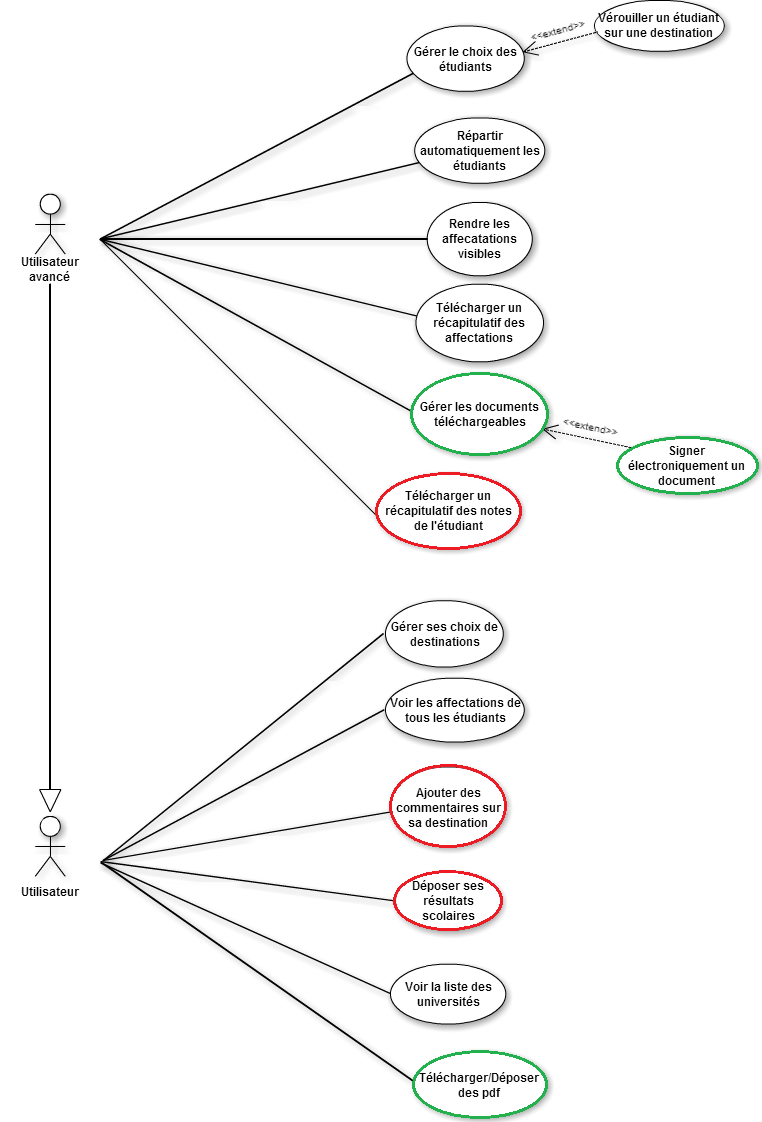
\includegraphics[scale=0.7]{images/useCaseDiagram.png}
	\caption{Diagramme de cas d'utilisation de l'application}
	\label{useCase}
\end{figure}